% -------------------------------------------------------------------
\documentclass[usepdftitle=false,10pt]{beamer}

%encodings
\usepackage[utf8]{inputenc}
\usepackage[OT1]{fontenc}

%some useful packages
\usepackage[]{mathrsfs}
\usepackage[]{amssymb}
\usepackage[]{amsmath}
\usepackage[]{acronym}
\usepackage[]{listings}
\usepackage[]{xcolor}
\usepackage[]{graphicx}
\usepackage[]{textcomp} %for tilde


%\usepackage[english]{babel}
%\usepackage[utf8]{inputenc}
%\usepackage{amsmath}
%\usepackage{graphicx}
%\usepackage{amsfonts}
%\usepackage[]{xcolor}
%\usepackage[]{graphicx}
%\usepackage[]{textcomp} %for tilde

\hypersetup{pdftitle={ViennaCL}, pdfauthor={Florian Rudolf}}


%% Listings package START
\usepackage{color}
\usepackage{listings}

\definecolor{darkblue}{rgb}{0,0,.6}
\definecolor{darkred}{rgb}{.6,0,0}
\definecolor{darkgreen}{rgb}{0,.6,0}
\definecolor{red}{rgb}{.98,0,0}
\definecolor{lightgrey}{rgb}{0.98,0.98,0.98}


\lstloadlanguages{C++}
\lstset{%
  language=C++,
  basicstyle=\small\ttfamily,
  commentstyle=\itshape\color{darkgreen},
  keywordstyle=\bfseries\color{darkblue},
  stringstyle=\color{darkred},
  showspaces=false,
  showtabs=false,
  columns=fixed,
  backgroundcolor=\color{lightgrey},
  numbers=none,
  frame=single,
  numberstyle=\tiny,
  breaklines=true,
  showstringspaces=false,
  xleftmargin=0.1cm,
  escapechar=|
}%

\lstset{emphstyle=\color{red}}

%% Listings package STOP








\renewcommand{\matrix}[1]{\boldsymbol{#1}}
\renewcommand{\vector}[1]{\boldsymbol{#1}}
\renewcommand{\d}{\mathrm{d}}
\newcommand{\domelem}[1]{\boldsymbol{\mathrm{#1}}}
\newcommand{\kB}{k_\mathrm{B}}
\newcommand{\VT}{V_\mathrm{T}}
\newcommand{\q}{\mathrm{q}}
\newcommand{\LandauO}{\mathcal{O}}
\newcommand{\Bullet}{$\triangleright$}
\newcommand{\black}{ }
\newcommand{\ViennaCL}{\texttt{ViennaCL}}

\newcommand{\TODO}[1]{{\color{red}\textbf{TODO: #1}}}

%\setlength{\fboxrule}{1pt}

%\renewcommand{\seriesdefault}{\bfdefault}
%\usepackage{helvet}

\graphicspath{{figures/}}           % in which folder all the figures are
\newcommand{\tn}   {\textnormal}

%\mode<presentation>

%\usetheme{Boadilla}
%\usecolortheme{albatross}
%\setbeamercolor{normal text}{bg=blue}
%\setbeamercolor{title}{fg=white}
%\setbeamercolor{structure}{fg=white}
%\setbeamertemplate{headline}
%{\begin{beamercolorbox}[left,sep=.3cm]{title in head/foot} \LARGE\insertsection \end{beamercolorbox}}
%\setbeamerfont{title}{size=\Large} % Der Titel auf der Titlepage
%\setbeamerfont{footline}{size=\scriptsize}
% Disable Navigation symbols:
%\setbeamertemplate{navigation symbols}{}

% table of contents, depth
\setcounter{tocdepth}{2}

% modify at will
\setbeamercovered{transparent}

\usetheme[height=0.3cm,width=0.8cm,shadow=false]{iue}


\author[Florian Rudolf]{Florian Rudolf}
%\author[Karl Rupp]{Karl Rupp}
%\author[Josef Weinbub]{Josef Weinbub}

\institute[TU Wien]
{ \footnotesize
  Institute for Microelectronics \\
  Institute for Analysis and Scientific Computing \\
  [1em]
  Technische Universit\"at Wien, Austria  
}

\title[ViennaCL]{  
\includegraphics[width=0.5\textwidth]{figs/viennacl-logo.pdf} \\ \\ The Vienna Computing Library \\ }
%\titlegraphic{
% \fcolorbox{black}{white}{ \hspace{1cm}
%    \includegraphics[keepaspectratio=true,height=1.5cm]{TUVienna.pdf} \hspace{2cm}
%    \includegraphics[keepaspectratio=true,height=1.5cm]{logo_asc.pdf} \hspace{2cm} 
%    \includegraphics[keepaspectratio=true,height=1.5cm]{logo_iue.pdf} \hspace{1cm}
%   }
%}
\date[CG Libs - Smart Libraries for Computer Graphics 2013]{ \footnotesize CG Libs - Smart Libraries for Computer Graphics 2013}

\setbeamertemplate{blocks}[default]
%\setbeamercolor{block title}{bg=}
\setbeamercolor{block body}{bg=}

\begin{document}
\newenvironment{equationfett}{\Large\begin{equation}}{\end{equation} \normalsize}
\newenvironment{boldalign}{\Large\begin{align*}}{\end{align*} \normalsize}
% -------------------------------------------------------------070605
% Dokumentbeginn 
% -------------------------------------------------------------------
\begin{frame}[plain]
 \frametitle{~}
 \titlepage
\end{frame}



\begin{frame}{Talk Overview}

  \begin{block}{Session 1}
    \begin{itemize}
    \item Introduction to ViennaCL
    \item How-To: ViennaCL Basics
    \end{itemize}
  \end{block}
  
  \begin{block}{Session 2}
    \begin{itemize}
    \item How-To: Advanced ViennaCL
    \item ViennaCL: Behind the curtain
    \end{itemize}
  \end{block}

\end{frame}



% ViennaCL Introduction


%%%%%%%%%%%%%%%%%%%%%%%%%%%%%%%%%%% Introduction to ViennaCL %%%%%%%%%%%%%%%%%%%%%%%%%%%%%%%%%%%%


\begin{frame}{ }
 \begin{center}
  \Large \textbf{Introduction to \ViennaCL}
 \end{center}
\end{frame}


\begin{frame}{Introduction to \ViennaCL}

\begin{block}{What to expect}
  \begin{itemize}
   \item What is ViennaCL
   \item OpenCL
   \item History of ViennaCL
   \item Goals of ViennaCL
   \item Installation of ViennaCL
  \end{itemize}
\end{block}

\end{frame}




\begin{frame}{What Is \ViennaCL?}

\begin{block}{What is it about the Name?}
\begin{itemize}
  \item The beautiful city of \textbf{Vienna}
  \item Open\textbf{CL}
\end{itemize}
\end{block}

\vspace{3.4cm}

\end{frame}


% \begin{frame}{What Is \ViennaCL?}
% 
% \begin{block}{What is it about the Name?}
% \begin{itemize}
%   \item The beautiful city of \textbf{Vienna}
%   \item Open\textbf{CL}
% \end{itemize}
% \end{block}
% 
% {
% \centering
% 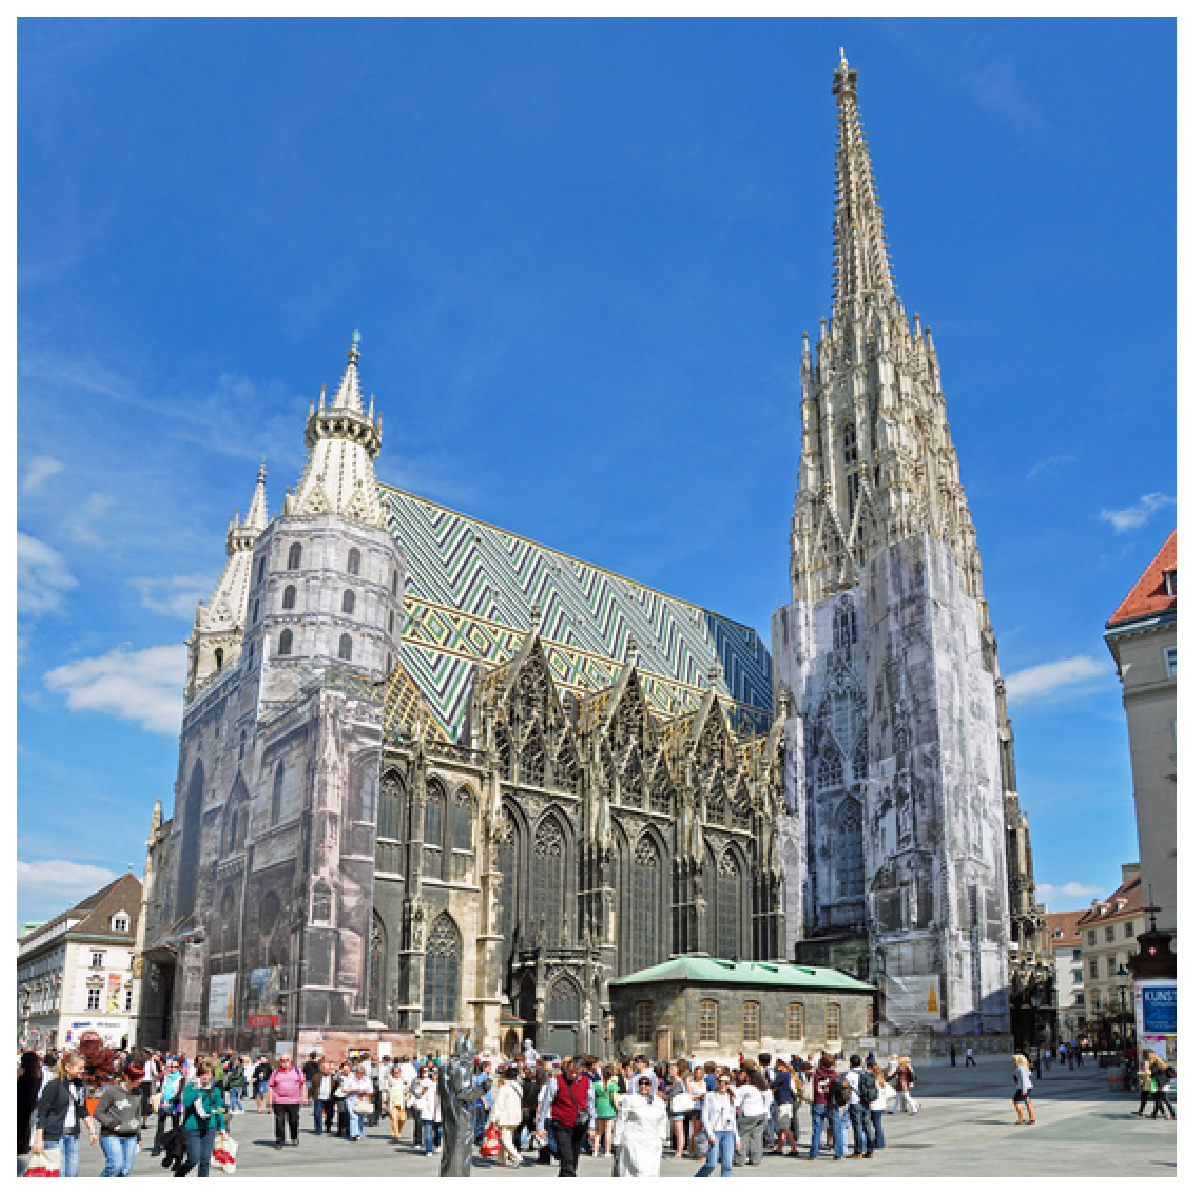
\includegraphics[width=0.3\textwidth]{figs/vienna.eps}
% }
% 
% \end{frame}


% \begin{frame}{What Is \ViennaCL?}
% 
% \begin{block}{What is it about the Name?}
% \begin{itemize}
%   \item The beautiful city of \textbf{Vienna}
%   \item Open\textbf{CL}
% \end{itemize}
% \end{block}
% 
% {
% \centering
% 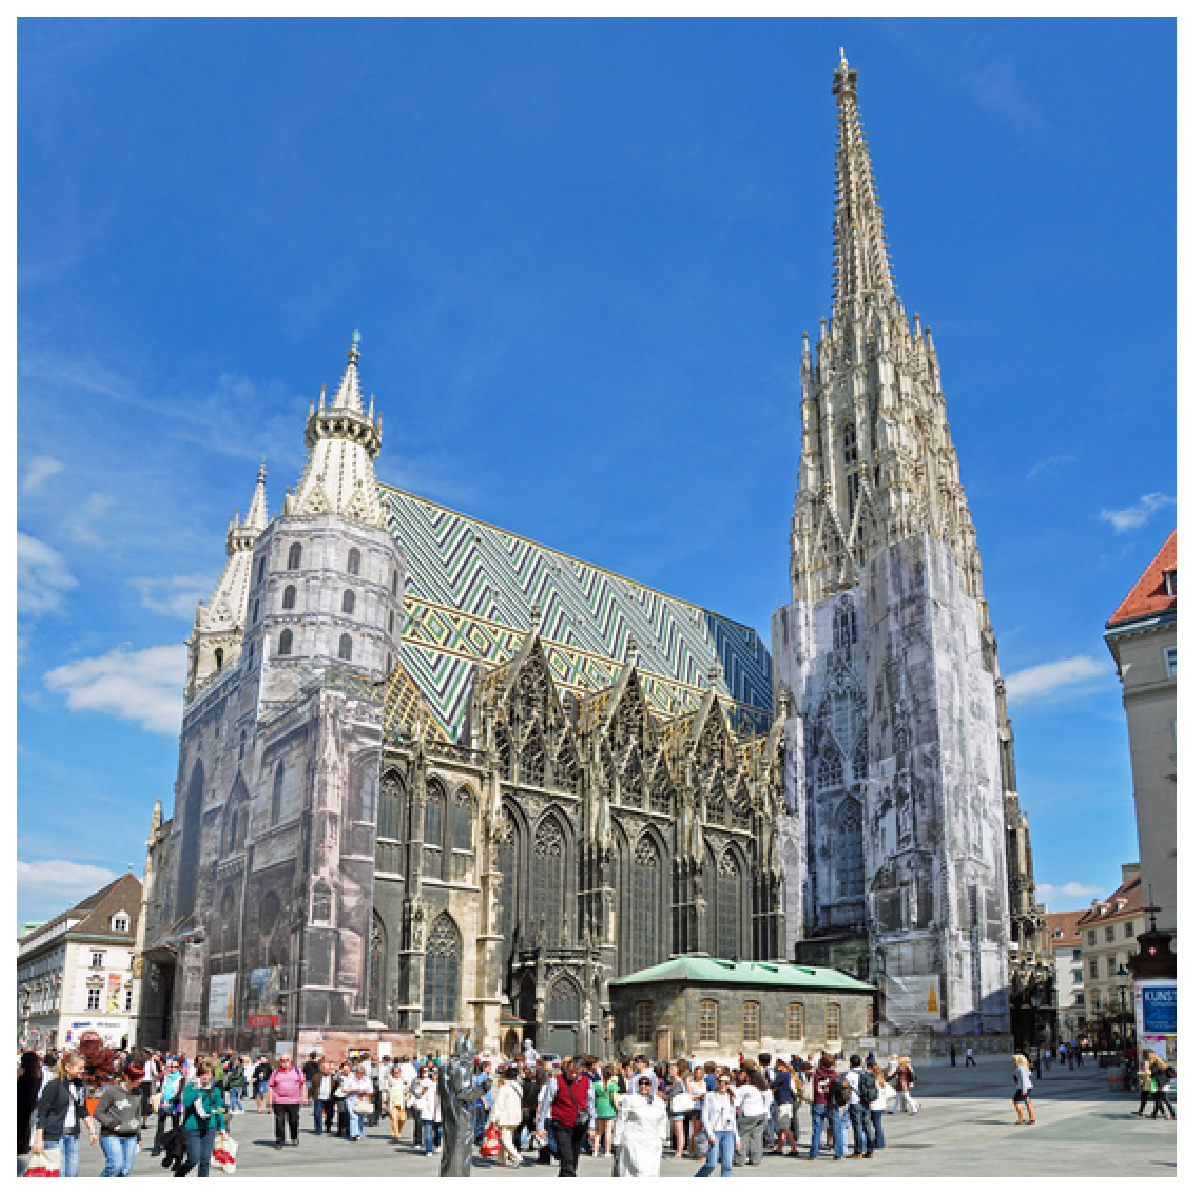
\includegraphics[width=0.3\textwidth]{figs/vienna.eps}
% \hspace{2cm}
% 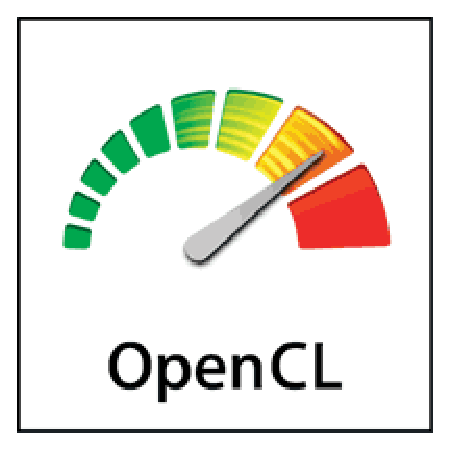
\includegraphics[width=0.3\textwidth]{figs/opencl_logo.eps}
% }
% 
% \end{frame}



\input{opencl}



\begin{frame}{History of \ViennaCL}

\begin{block}{2010}
  \begin{itemize}
   \item April: Roots in the Master's Thesis of Florian Rudolf
   \item May 28th: ViennaCL 1.0.0 released
   \item November: 1000th download
   \item December: ViennaCL 1.1.0 \\(BLAS level 3, refurbished OpenCL backend)
  \end{itemize}
\end{block}

\vspace*{2.49cm}
\end{frame}



\begin{frame}{History of \ViennaCL}

\begin{block}{2010}
  \begin{itemize}
   \item April: Roots in the Master's Thesis of Florian Rudolf
   \item May 28th: ViennaCL 1.0.0 released
   \item November: 1000th download
   \item December: ViennaCL 1.1.0 \\(BLAS level 3, refurbished OpenCL backend)
  \end{itemize}
\end{block}

\begin{block}{2011}
  \begin{itemize}
   \item March: Accepted for Google Summer of Code
   \item December: ViennaCL 1.2.0 \\ (AMG, SPAI, FFT, QR, graph algorithms, structured matrices)
  \end{itemize}
\end{block}

\end{frame}



\begin{frame}{History of \ViennaCL}

\begin{block}{2012}
  \begin{itemize}
   \item March: Accepted for Google Summer of Code
   \item May: Tutorial at NVIDIA GTC 2012
   \item May: ViennaCL 1.3.0 \\ (ranges and slices, Automated OpenCL kernels, eigen values, ILU0, SVD)
   \item December: ViennaCL 1.4.0 \\ (CUDA and host backend, initializer types)
  \end{itemize}
\end{block}

\vspace{2.07cm}

\end{frame}


\begin{frame}{History of \ViennaCL}

\begin{block}{2012}
  \begin{itemize}
   \item March: Accepted for Google Summer of Code
   \item May: Tutorial at NVIDIA GTC 2012
   \item May: ViennaCL 1.3.0 \\ (ranges and slices, Automated OpenCL kernels, eigen values, ILU0, SVD)
   \item December: ViennaCL 1.4.0 \\ (CUDA and host backend, initializer types)
  \end{itemize}
\end{block}

\begin{block}{2013}
  \begin{itemize}
   \item May: Accepted for Google Summer of Code
   \item June: Tutorial at CGLibs
  \end{itemize}
\end{block}

\end{frame}


% \begin{frame}{History of \ViennaCL}
% 
% \TODO{Achievement unlocked: Historian}
% 
% \end{frame}



\begin{frame}{Goals of \ViennaCL}

  \begin{block}{About}
   \begin{itemize}
    \item High-level linear algebra C++ library
    \item OpenMP, OpenCL, and CUDA backends
    \item Header-only
    \item Multi-platform
   \end{itemize}
  \end{block}

  \vspace*{-2.3cm}
  \begin{flushright}
   \includegraphics[width=0.4\textwidth]{figs/ViennaCL-arch.png}
  \end{flushright}

  \vspace*{-0.7cm}
  \begin{block}{Dissemination}
    \begin{itemize}
     \item Free Open-Source MIT (X11) License
     \item http://viennacl.sourceforge.net/
     \item 50-100 downloads per week
    \end{itemize}   
  \end{block}

  \begin{block}{Design Rules}
   \begin{itemize}
    \item Reasonable default values
    \item Compatible to Boost.uBLAS whenever possible 
    \item In doubt: clean design over performance
   \end{itemize}
  \end{block}

\end{frame}



\begin{frame}{Goals of \ViennaCL}

  \begin{block}{Core features}
    \begin{itemize}
     \item Linear algebra, BLAS
     \item Solver (direct and iterative)
     \item Preconditioners
    \end{itemize}   
  \end{block}
     
  \begin{block}{Additional features}
    \begin{itemize}
     \item Fast Fourier Transform
     \item Eigenvalue computations
     \item QR factorization
     \item Bandwidth reduction
     \item Nonnegative matrix factorization
    \end{itemize}   
  \end{block}

\end{frame}



\begin{frame}{Goals of \ViennaCL}

  \begin{block}{Interfaces to other libraries}
    \begin{itemize}
     \item Boost.uBLAS
     \item Eigen
     \item MTL4
    \end{itemize}   
  \end{block}

  \begin{block}{Backends}
   \begin{itemize}
    \item CPU
    \item OpenCL
    \item CUDA
   \end{itemize}
  \end{block}

  \begin{block}{C++ library}
   \begin{itemize}
    \item Generic free functions
    \item Expression templates
   \end{itemize}
  \end{block}

\end{frame}



\begin{frame}{Installation of \ViennaCL}

  \begin{block}{Three Steps}
    \begin{itemize}
     \item Download from http://viennacl.sourceforge.net/
     \item Unzip
     \item Copy source folder
    \end{itemize}   
  \end{block}

  \begin{block}{Dynamic Library?}
    \begin{itemize}
     \item ViennaCL is header-only
     \item Linking depends on used backend (OpenMP, OpenCL, CUDA)
    \end{itemize}
  \end{block}

  \begin{block}{Sample Applications}
    \begin{itemize}
     \item 22 tutorials
     \item $\hphantom{0}$7 benchmarks
     \item about 35 tests
    \end{itemize}
  \end{block}

\end{frame}



% ViennaCL Basics
\input{viennacl_basics}

% Advanced ViennaCL
\input{viennacl_advanced}

% ViennaCL: behind the curtain

\begin{frame}{ }
 \begin{center}
  \Large \textbf{\ViennaCL : Behind the curtain}
 \end{center}
\end{frame}


\begin{frame}{\ViennaCL : Behind the curtain}

\begin{block}{What to expect}
  \begin{itemize}
   \item Backends
   \item OpenCL kernel management
   \item Extending ViennaCL
   \item ViennaCL and OpenGL
   \item Summary
  \end{itemize}
\end{block}

\end{frame}



\begin{frame}{\ViennaCL : Behind the curtain}

\begin{block}{Backends}
  \begin{itemize}
   \item There is more than OpenCL
   \item CUDA from NVIDIA
   \item OpenACC
   \item Each framework has advantages and disadvantages
  \end{itemize}
\end{block}

\end{frame}



\begin{frame}[fragile]
\frametitle{Backends}
 \begin{block}{OpenCL}
  { \lstset{ basicstyle=\scriptsize\ttfamily } \begin{lstlisting}
const char *kernel_string =
"__kernel void mykernel(__global double *buffer) {
  buffer[get_global_id(0)] = 42.0;
};";   

int main() {
  ...
  cl_program my_prog = clCreateProgramWithSource(
         my_context,1,&kernel_string,&source_len,&err);
  clBuildProgram(my_prog,0,NULL,NULL,NULL,NULL);
  cl_kernel my_kernel = clCreateKernel(my_prog,
                          "mykernel",&err);
  clSetKernelArg(my_kernel,0,sizeof(cl_mem),&buffer);
  clEnqueueNDRangeKernel(queue,my_kernel,1,NULL,
               &global_size,&local_size,0,NULL,NULL);
} 
  \end{lstlisting} }

  \begin{itemize}
   \item Additional boilerplate code required (low-level API)
   \item Broad hardware support (separate SDKs)
   \item No more development effort from NVIDIA
  \end{itemize}
 \end{block}

\end{frame}



\begin{frame}[fragile]
\frametitle{Backends}
 \begin{block}{NVIDIA CUDA}
  { \lstset{ basicstyle=\scriptsize\ttfamily } \begin{lstlisting}
// GPU kernel:
__global__ void kernel(double *buffer)
{
  int idx = blockIdx.x * blockDim.x + threadIdx.x;
  buffer[idx] = 42.0;
}

// host code:
int main()
{ 
  ...
  cudaMalloc((void**)&buffer,size);
  kernel<<<blocknum, blockdim>>>(buffer);
  ...
}
  \end{lstlisting} }

  \begin{itemize}
   \item Almost no additional code required
   \item Vendor-lock
   \item Relies on \lstinline|nvcc| being available
  \end{itemize}
 \end{block}

\end{frame}



\begin{frame}[fragile]
\frametitle{Backends}
 \begin{block}{OpenACC}
  { \lstset{ basicstyle=\scriptsize\ttfamily } \begin{lstlisting}
void func(...) {
  #pragma acc data pcopyin(A[0:size][0:size])
  {
    #pragma acc kernels loop
    for(int i=0; i< size; i++)
      for(int j=0; j < size; j++)
        A[i][j] = 42;
  }
}

int main()
{
  double A[1337][1337];
  func(A);
}
  \end{lstlisting} }

  \begin{itemize}
   \item Simple OpenMP-type pragma annotations
   \item Compiler support?
   \item Insufficient control over memory transfers?
  \end{itemize}
 \end{block}

\end{frame}



\begin{frame}{Backends}

\begin{block}{What to use?}
  \begin{itemize}
    \item Why choose one when we can support all?
  \end{itemize}
\end{block}

\begin{block}{ViennaCL has a backend layer}
  \begin{itemize}
    \item Backend is responsible for hardware interaction
    \item Not only OpenCL anymore
    \item Since ViennaCL 1.4.0
  \end{itemize}
\end{block}

\begin{block}{Different backends supported}
  \begin{itemize}
    \item OpenCL
    \item OpenMP
    \item CUDA
  \end{itemize}
\end{block}

\end{frame}



\begin{frame}[fragile]
\frametitle{Backends}

\begin{block}{Backend support has to be enabled explicitly}
\vspace{0.83cm}
\begin{lstlisting}
viennacl::vector<float> v1, v2;
v1 += v2;
\end{lstlisting}

  \begin{itemize}
   \item CPU used!
  \end{itemize}
\end{block}

\end{frame}



\begin{frame}[fragile]
\frametitle{Backends}

\begin{block}{Backend support has to be enabled explicitly}
\begin{lstlisting}
#define VIENNACL_WITH_OPENCL

viennacl::vector<float> v1, v2;
v1 += v2;
\end{lstlisting}

  \begin{itemize}
   \item Now we are using OpenCL
  \end{itemize}
\end{block}

\end{frame}



\begin{frame}{Backends}

Lets take a look!

\end{frame}




\begin{frame}[fragile]
\frametitle{Backends}

 \begin{block}{Vector Addition}
  \begin{itemize}
   \item Memory buffers can switch memory domain at runtime
  \end{itemize}
  \begin{lstlisting}
void avbv(...) { // x = y + z
  switch (active_handle_id(x))
  {
    case MAIN_MEMORY:
      host_based::avbv(...);
      break;
    case OPENCL_MEMORY:
      opencl::avbv(...);
      break;
    case CUDA_MEMORY:
      cuda::avbv(...);
      break;
    default: 
      raise_error();
  }
}
\end{lstlisting}
 \end{block}

\end{frame}



\begin{frame}[fragile]
\frametitle{Internals}

 \begin{block}{Memory Buffer Migration}
  \begin{lstlisting}
  vector<double> x = zero_vector<double>(42);

  memory_types src_memory_loc = memory_domain(x);
  switch_memory_domain(x, MAIN_MEMORY);
  /* do work on x in main memory here */
  switch_memory_domain(x, src_memory_loc);
\end{lstlisting}

  \begin{center}
    \includegraphics[width=0.6\textwidth]{figs/ViennaCL-arch.png}
  \end{center}
 \end{block}

\end{frame}



\begin{frame}[fragile]
\frametitle{Backends}

\begin{block}{Memory buffer switching at runtime}
\begin{lstlisting}
#define VIENNACL_WITH_OPENCL
#define VIENNACL_WITH_OPENMP

viennacl::vector<float> v1, v2;

switch_memory_domain(v1, MAIN_MEMORY);
switch_memory_domain(v2, MAIN_MEMORY);

v1 += v2; \\ working on CPU with OpenMP

switch_memory_domain(v1, OPENCL_MEMORY);
switch_memory_domain(v2, OPENCL_MEMORY);

v1 += v2; \\ working on GPU with OpenCL
\end{lstlisting}
\end{block}

\end{frame}








\begin{frame}{OpenCL kernel management}

\begin{block}{Best kernel implementations depend on target hardware}
  \begin{itemize}
    \item NVIDIA, AMD, Intel
  \end{itemize}
\end{block}

\begin{block}{Best work group size depends on target hardware}
  \vspace{0.3cm}
  \begin{tabular}{l|llll|llll}
    \multicolumn{5}{c}{ \hspace{0.6cm} NVIDIA} & \multicolumn{4}{c}{AMD} \\
    & 32  & 64  & 128 & 256 & 32 & 64 & 128 & 256 \\
    \hline
    64  & 191 & 151 & 174 & 193 & 324 & 262 & 256 & 249 \\
    128 & 194 & 177 & \textbf{195} & 214 & 357 & 290 & \textbf{272} & \textbf{247} \\
    256 & 161 & 164 & 195 & 214 & 307 & 264 & 256 & 248 \\
    512 & \textbf{145} & 157 & 198 & 211 & 282 & 255 & 258 & 253 \\
  \end{tabular}
  \vspace{0.3cm}
  \\Execution times for sparse matrix-vector product in milliseconds
\end{block}

\end{frame}



\begin{frame}[fragile]
\frametitle{OpenCL kernel management}

\begin{block}{Kernel parameter tuning}
  \begin{itemize}
    \item Default number of work groups = 128
    \item Default number of work items per work group = 128
    \item Automatic tuning environment $\Rightarrow$ XML file
  \end{itemize}
\end{block}

\begin{block}{How to use kernel parameters}
\begin{lstlisting}
using namespace viennacl;
using viennacl::io;

read_kernel_parameters< vector<float> >
    ("float_vector_parameters.xml");
read_kernel_parameters< matrix<float> >
    ("float_matrix_parameters.xml");
read_kernel_parameters< compressed_matrix<float> >
    ("float_sparse_parameters.xml");
\end{lstlisting}
\end{block}

\end{frame}



\begin{frame}{OpenCL kernel management}

\begin{block}{ViennaCL expression template don't cover all operations}
  \begin{itemize}
    \item Sample operation: $\mathbf{x} = \mathbf{A} \times \bigl[ (\mathbf{y} \cdot (\mathbf{y}+\mathbf{z}))\mathbf{y} + \mathbf{z} \bigr]$
  \end{itemize}
\end{block}

\begin{block}{Automated kernel generation}
  \begin{itemize}
    \item Supported since ViennaCL 1.3.0
    \item Experimental support
  \end{itemize}
\end{block}

\begin{block}{Symbolic variables}
  \begin{itemize}
    \item Operation is defined with C++ symbolic variables
    \item Custom kernel object is generated
  \end{itemize}
\end{block}

\end{frame}



\begin{frame}[fragile]
\frametitle{OpenCL kernel management}

\begin{block}{Automated kernel generation}
  \begin{itemize}
    \item Sample operation: $\mathbf{x} = \mathbf{A} \times \bigl[ (\mathbf{y} \cdot (\mathbf{y}+\mathbf{z}))\mathbf{y} + \mathbf{z} \bigr]$
  \end{itemize}
  \begin{lstlisting}
// Instantiation of the symbolic variables
symbolic_vector<NumericType, 0> sX;
symbolic_matrix<NumericType, 1> sA;
symbolic_vector<NumericType, 2> sY;
symbolic_vector<NumericType, 3> sZ;

//Creation of the custom operation
custom_operation my_op(
    sX = prod(sA, inner_prod(sY, sY+sZ) * sY + sZ),
    "operation_name" );
  \end{lstlisting}
\end{block}

\end{frame}



\begin{frame}[fragile]
\frametitle{OpenCL kernel management}

\begin{block}{Automated kernel execution}
  \begin{lstlisting}
viennacl::vector<NumericType> x, y, z;
viennacl::matrix<NumericType> A;
  
// fill data here
  
//Execution of the custom operation
viennacl::ocl::enqueue(my_op(x,A,y,z));
  \end{lstlisting}
\end{block}

\end{frame}





\begin{frame}[fragile]
\frametitle{Extending ViennaCL}

\begin{block}{Not Everything Covered by ViennaCL}
 \begin{itemize}
  \item Complicated vector expressions in a single compute kernel
 \end{itemize}
\end{block}

\begin{block}{Direct OpenCL Kernel Handling is a Pain}
  \begin{lstlisting}
const char * my_kernel_sources = 
"__kernel void element_prod(\n"
"          __global const float * vec1,\n"
"          __global const float * vec2, \n"
"          __global float * result,\n"
"          unsigned int size) \n"
"{ \n"
"  for (unsigned int i = get_global_id(0);  \n"
"                    i < size;  \n"
"                    i += get_global_size(0))\n"
"    result[i] = vec1[i] * vec2[i];\n"
"};\n";
  \end{lstlisting}
\end{block}

\end{frame}


\begin{frame}[fragile]
\frametitle{Extending ViennaCL}

\begin{block}{The OpenCL Way (error checks and casts omitted)}
  { \lstset{ basicstyle=\scriptsize\ttfamily } \begin{lstlisting}
size_t source_len = std::string(my_compute_program).length();
cl_program my_prog = clCreateProgramWithSource(my_context, 1, 
                         &my_kernel_sources, &source_len, &err);
err = clBuildProgram(my_prog, 0, NULL, NULL, NULL, NULL);

const char * kernel_name = "element_prod";
cl_kernel my_kernel = clCreateKernel(my_prog, kernel_name, &err);

err = clSetKernelArg(my_kernel, 0, sizeof(cl_mem), &mem_vec1);
err = clSetKernelArg(my_kernel, 1, sizeof(cl_mem), &mem_vec2);
err = clSetKernelArg(my_kernel, 2, sizeof(cl_mem), &mem_result);
err = clSetKernelArg(my_kernel, 3, sizeof(unsigned int), &vsize);
err = clEnqueueNDRangeKernel(queues[0], my_kernel, 1, NULL, 
                       &global_size, &local_size, 0, NULL, NULL);
  \end{lstlisting} }
\end{block}

 \begin{block}{Issues}
  \begin{itemize}
   \item Access \texttt{my\_kernel} at some other location in an application?
   \item What to do with \texttt{my\_prog}?
  \end{itemize}
 \end{block}

  

\end{frame}



\begin{frame}[fragile]
\frametitle{Extending ViennaCL}

\begin{block}{The ViennaCL Way (namespaces omitted)}
  {\black \begin{lstlisting}
program & my_prog = 
  current_context().add_program(my_kernel_sources, 
                                "my_program");
kernel & my_kernel = my_prog.add_kernel("element_prod");
enqueue(my_kernel(vec1, vec2, result, vec1.size()) );
  \end{lstlisting} }
\end{block}

\begin{block}{At any other Location within the Application}
  {\black \begin{lstlisting}
kernel & my_kernel = get_kernel(
    "my_program", "element_prod");
viennacl::ocl::enqueue(
    my_kernel(vec1, vec2, result, vec1.size()) );
  \end{lstlisting} }
\end{block}

  \begin{block}{Allows for Adding Missing Functionality Easily}
    \begin{itemize}
     \item A bit of OpenCL knowledge required
    \end{itemize}
  \end{block}

\end{frame}



\begin{frame}[fragile]
\frametitle{Extending ViennaCL}

\begin{block}{Integrate ViennaCL into User-Environment}
 \begin{itemize}
  \item User-provided context, queue and device
 \end{itemize}
\end{block}

  \begin{lstlisting}
cl_context my_context = ...; //a context
cl_device_id my_device = ...; //a device in my_context
cl_command_queue my_queue = ...; //a queue for my_device
// supply existing context 'my_context' with one device 
// and one queue to ViennaCL using id '0':
viennacl::ocl::setup_context(0, my_context, my_device, my_queue);
  \end{lstlisting}

\begin{block}{Wrapping Memory Buffers}
  \begin{lstlisting}
   cl_mem my_memory = ...;
   viennacl::vector<float> my_vec(my_memory, 10);
  \end{lstlisting}
 \begin{itemize}
  \item Use ViennaCL operations as usual
 \end{itemize}

\end{block}

\end{frame}



\begin{frame}{ViennaCL and OpenGL}

\begin{block}{ViennaCL and OpenGL}
  \begin{itemize}
    \item Since OpenCL 1.1: OpenGL interoperability
    \item With own OpenCL context: easy task
  \end{itemize}
\end{block}

\begin{block}{Workflow}
  \begin{itemize}
    \item Setup OpenGL and OpenCL
    \item Create OpenGL buffer and OpenCL memory object
    \item Pass OpenCL memory object to ViennaCL
    \item Do ViennaCL magic
    \item Use data in OpenGL
  \end{itemize}
\end{block}

\end{frame}



\begin{frame}[fragile]
\frametitle{ViennaCL and OpenGL}

\begin{block}{Setup OpenGL context (simple glut-glew magic)}
  \begin{lstlisting}
glutInit(&argc, argv);
    
glutInitDisplayMode(...);
glutInitWindowPosition(100,100);
glutInitWindowSize(1600,800);
glutCreateWindow("CL - GL");
    
glewInit();
  \end{lstlisting}
\end{block}

\end{frame}



\begin{frame}[fragile]
\frametitle{ViennaCL and OpenGL}

\begin{block}{Setup OpenCL context with OpenGL interoperability support}
  \begin{lstlisting}
cl_context_properties properties[] = {
    CL_GL_CONTEXT_KHR, (cl_context_properties)
        glXGetCurrentContext(),
    CL_GLX_DISPLAY_KHR, (cl_context_properties)
        glXGetCurrentDisplay(),
    CL_CONTEXT_PLATFORM, (cl_context_properties)
        viennacl::ocl::get_platforms()[0].id(),
    0};
    
cl_device_id my_device =
    viennacl::ocl::current_device().id();
        
cl_context my_context = clCreateContext(properties, 1,
    &my_device, NULL, NULL, &err);
cl_command_queue my_queue = clCreateCommandQueue(
    my_context, my_device, 0, &err );
  \end{lstlisting}
\end{block}

\end{frame}


\begin{frame}[fragile]
\frametitle{ViennaCL and OpenGL}

\begin{block}{Setup OpenCL context with OpenGL interoperability support}
  \begin{lstlisting}
cl_context_properties properties[] = {
    |\color{red}CL\_GL\_CONTEXT\_KHR, (cl\_context\_properties)|
        |\color{red}glXGetCurrentContext()|,
    |\color{red}CL\_GLX\_DISPLAY\_KHR, (cl\_context\_properties)|
        |\color{red}glXGetCurrentDisplay()|,
    |\color{red}CL\_CONTEXT\_PLATFORM, (cl\_context\_properties)|
        |\color{red}viennacl::ocl::get\_platforms()[0].id()|,
    0};
    
cl_device_id my_device =
    viennacl::ocl::current_device().id();
        
cl_context my_context = clCreateContext(properties, 1,
    &my_device, NULL, NULL, &err);
cl_command_queue my_queue = clCreateCommandQueue(
    my_context, my_device, 0, &err );
  \end{lstlisting}
\end{block}

\end{frame}



\begin{frame}[fragile]
\frametitle{ViennaCL and OpenGL}

\begin{block}{Setting up ViennaCL for our context}
  \begin{lstlisting}
viennacl::ocl::setup_context( 
    0,          // the ViennaCL context ID
    my_context, // our context with OpenGL interoperability
    my_device,  // the device we are working on
    my_queue ); // the command queue for our context
    
// tell ViennaCL that we want to use our context
viennacl::ocl::switch_context( 0 );
  \end{lstlisting}
\end{block}

\end{frame}




\begin{frame}[fragile]
\frametitle{ViennaCL and OpenGL}

\begin{block}{Create OpenGL buffer and OpenCL memory object}
  \begin{lstlisting}
glGenBuffers(1, &gl_buffer);
glBindBuffer( GL_PIXEL_UNPACK_BUFFER, gl_buffer );
glBufferData( GL_PIXEL_UNPACK_BUFFER, size, NULL, GL_DYNAMIC_COPY );

cl_mem cl_buffer = clCreateFromGLBuffer(my_context, CL_MEM_READ_WRITE, gl_buffer, &err);
  \end{lstlisting}
\end{block}

\end{frame}



\begin{frame}[fragile]
\frametitle{ViennaCL and OpenGL}

\begin{block}{ViennaCL magic}
  \begin{lstlisting}
// Create viennacl vector from OpenCL memory
viennacl::vector<float> my_vec(cl_buffer, size);

// Acquire memory object for write read/write operation
clEnqueueAcquireGLObjects(my_queue, 1, &cl_buffer,
    0, NULL, NULL);

// copy CPU data to ViennaCL
viennacl::copy( tmp_vec, my_vec );
// doing some stuff
my_vec *= 0.5f;

// Release memory object
clEnqueueReleaseGLObjects(my_queue, 1, &cl_buffer,
    0, NULL, NULL);
  \end{lstlisting}
\end{block}

\end{frame}



\begin{frame}[fragile]
\frametitle{ViennaCL and OpenGL}

\begin{block}{ViennaCL magic}
  \begin{lstlisting}
// Create viennacl vector from OpenCL memory
viennacl::vector<float> my_vec(cl_buffer, size);

// Acquire memory object for write read/write operation
|\color{red}clEnqueueAcquireGLObjects(my\_queue, 1, \&cl\_buffer,|
    |\color{red}0, NULL, NULL);|

// copy CPU data to ViennaCL
viennacl::copy( tmp_vec, my_vec );
// doing some stuff
my_vec *= 0.5f;

// Release memory object
|\color{red}clEnqueueReleaseGLObjects(my\_queue, 1, \&cl\_buffer,|
    |\color{red}0, NULL, NULL);|
  \end{lstlisting}
\end{block}

\end{frame}



\begin{frame}{ViennaCL and OpenGL}

Lets take a look at this example

\end{frame}



\begin{frame}{Summary}
\begin{block}{What have we learned?}
  \begin{itemize}
   \item ViennaCL has different backends
   \item How to enable and use backends
   \item OpenCL management in ViennaCL
   \item How to use an own OpenCL kernel with ViennaCL
   \item How to provide own OpenCL contexts
   \item ViennaCL works with OpenGL!
   \item How to use ViennaCL to work with OpenGL
  \end{itemize}
\end{block}
\end{frame}


% \begin{frame}{Summary}
% \TODO{Achievement unlocked: ViennaCL god}
% \end{frame}







% Conclustion




\begin{frame}{Acknowledgements}

 \begin{minipage}{0.5\textwidth}
  \begin{block}{Contributors}
    \begin{itemize}
     \item Thomas Bertani
     \item Evan Bollig
     \item Philipp Grabenweger
     \item Volodymyr Kysenko
     \item Nikolay Lukash
     \item G\"unther Mader
     \item Vittorio Patriarca
     \item Florian Rudolf
     \item Astrid Rupp
     \item \textbf{Karl Rupp}
     \item Philippe Tillet
     \item Markus Wagner
     \item Josef Weinbub
     \item Michael Wild
    \end{itemize}
  \end{block}
 \end{minipage}
 \begin{minipage}{0.4\textwidth}
  \includegraphics[width=0.65\textwidth]{figs/gsoc2011.png}
  \vspace*{0.2cm} \\
  \includegraphics[width=0.65\textwidth]{figs/gsoc2012.png}
  \vspace*{0.2cm} \\
  \includegraphics[width=0.65\textwidth]{figs/nvidia_logo_black.png}
  \vspace*{0.2cm} \\
  \includegraphics[width=0.65\textwidth]{figs/amd-logo.png}
 \end{minipage}

\end{frame}



\begin{frame}{Summary}
 
 \begin{block}{High-Level C++ Approach of ViennaCL}
  \begin{itemize}
   \item Convenience of single-threaded high-level libraries (Boost.uBLAS)
   \item Header-only library for simple integration into existing code
   \item MIT (X11) license
   \item \centering http://viennacl.sourceforge.net/
  \end{itemize}
 \end{block}

 \begin{block}{Selected Features}
  \begin{itemize}
   \item Backends: OpenMP, OpenCL, CUDA
   \item Iterative Solvers: CG, BiCGStab, GMRES
   \item Preconditioners: AMG, SPAI, ILU, Jacobi
   \item BLAS: Levels 1-3
   \item 
  \end{itemize}
 \end{block}

\end{frame}


%%
%%
%%  Part 1: Algorithmic Aspects
%%
%%

%\input{algorithmic}


%%
%%
%%  Part 2: Software Aspects
%%
%%

%\input{software}


%%
%%
%%  Part 3: Current and Future Topics
%%
%%

%\input{future}




\end{document}

